\subsection{Quadratische Funktionen}
Die n"achst einfachsten Funktionen nach den linearen stellen die so genannten quadratischen Funktionen dar. Sie werden auch als Parabelgleichungen bezeichnet. Ihren Namen verdanken diese Funktionen der Tatsache, dass ihre Variable zumindest einmal quadratisch und niemals mit einem h"oheren Exponenten als $2$ in die Gleichung mit eingeht.

\subsubsection{Die Normalparabel}
Die Normalparabel besitzt die Formel 
\begin{equation*}
f(x) = x^2
\end{equation*}
Sie ist eine nach oben ge"offnete, achsensymmetrische Kurve dar, deren niedrigster Punkt (Scheitel) $S$ im Ursprung des Koordinatensystems $(0,0)$ liegt.

%Siehe: Verschieben einer Funktion
%\subsubsection{Verschieben einer Parabel}
%Wollen wir eine 
%Eine Parabel l"asst sich um den Wert $x_s$ in $x$-Richtung verschieben, indem man diesen Wert von der Variable $x$ subtrahiert, daraus folgt:\\
%$f(x)=(x-x_s)^2$\vspace{0.25 cm}\flushleft
%Durch Addition des gesamten Terms mit dem Wert $y_s$ wird die Parabel um den gleichen Wert in y-Richtung verschoben.\\
%Die Gleichung der Parabel lautet nun wie folgt:\\
%$f(x)=(x-x_s)^2+y_s$\\
%Ihr Scheitel besitzt die Koordinaten $S(x_s,y_s)$.

\subsubsection{Stauchen und Strecken}
Durch Multiplizieren der Normalparabel mit einer konstanten $a$ l"asst sich die Kurve stauchen oder strecken. $f(x)=a \cdot x^2$ Ist der Betrag von $a$ kleiner $1$, so wird die Parabel gestaucht. Ist er gr"o"ser $1$, so wird sie gestreckt. Dar"uber hinaus wird die Funktion durch einen negativen Wert von a an der $x$-Achse gespiegelt und die Parabel ist somit nach unten ge"offnet.
\begin{figure}[h!]
\begin{center}
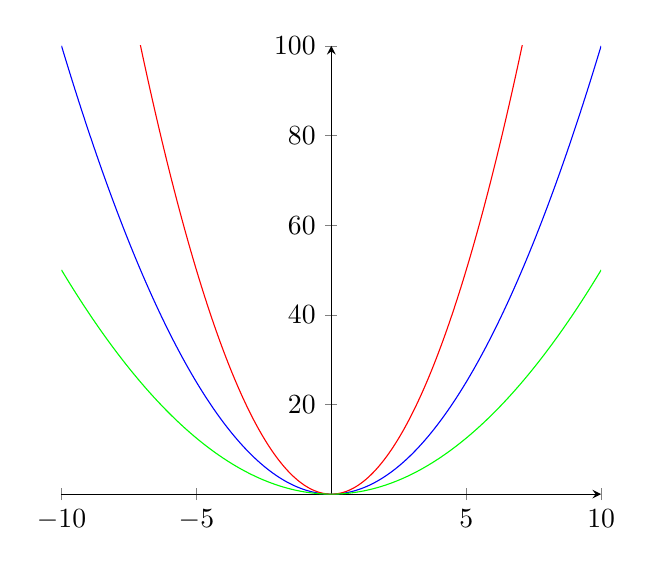
\begin{tikzpicture}[scale = 1.0]
    \begin{axis}[
        domain=-10:10,
        xmin=-10, xmax=10,
        ymin=-0, ymax=100,
        samples=400,
        axis y line=center,
        axis x line=middle,
    ]
    	   \addplot+[mark=none, color=blue] { x*x};
        \addplot+[mark=none, color=red] {2 * x*x};
         \addplot+[mark=none, color=green] {0.5 * x*x};
    \end{axis}
\end{tikzpicture}
\end{center}
\caption{Normalparabel, gestreckte und gestauchte Normalparabel}
\end{figure}

\subsubsection{Die Scheitelform}
Durch Kombination von Stauchung/Streckung und Verschiebung erh"alt man die so genannte Scheitelform: 
\begin{equation*}
f(x)=a(x-x_s)^2+y_s
\end{equation*}
Mithilfe dieser Funktion lassen sich alle Arten quadratischer Funktionen darstellen. Au"serdem lassen sich die Koordinaten des Scheitels, der Stauchungs- bzw. Streckungsfaktor der Funktion, sowie die Frage, ob sie nach oben oder unten ge"offnet ist, auf einfachste Weise bestimmen.

\subsubsection{Die Normalform einer quadratischen Gleichung}
Multipliziert man die Scheitelform aus, so erh"alt man 
\begin{equation*}
f(x)=a \cdot x^2-2 \cdot a \cdot x_sx+x_s^2+y_s.
\end{equation*}
Ersetzt man nun die konstanten Werte $-2ax_s$ durch $b$ und $x_s^2+y_s$ durch $c$, so erh"alt man die \textbf{Normalform} quadratischer Gleichungen:
\begin{equation*}
f(x)=a \cdot x^2+b \cdot x+c
\end{equation*}

\subsubsection{Die binomischen Formeln}
Die binomischen Formeln sind das Ergebnis des Ausmultiplizierens, hat man sie jedoch im Kopf so spart man viel Zeit.
\begin{enumerate}
\item $(a+b)^2=a^2+2ab+b^2$
\item $(a-b)^2=a^2-2ab+b^2$
\item $(a+b)(a-b)=a^2-b^2$
\end{enumerate}

\subsubsection{Die quadratische Erg"anzung}
Will man zum Beispiel zur Bestimmung des Scheitelpunktes die Normalform der quadratischen Gleichung in die Scheitelform umwandeln, so geht dies unter anderem mithilfe der so genannten quadratischen Erg"anzung. Zun"achst einmal besitzt man eine quadratische Gleichung in der Normalform.\\
Im Folgenden wird nun die Scheitelform der Funktion $f(x)=3x^2-6x-24$ berechnet:\\
Der erste Schritt hierf"ur ist das Ausklammern der Konstante "'a"', in unserem Fall der 3:\\
$f(x)=3(x^2-2x-8)$\\
Schaut man sich nun den Term innerhalb der runden Klammern genauer an, so kann man eine gewisse "Ahnlichkeit mit der ersten, bzw. zweiten binomischen Formel feststellen.\\
Deshalb folgt nun auch der wichtigste Schritt, die eigentliche quadratische Erg"anzung. Wir erg"anzen die Formel nun so, dass wir eine der beiden binomischen Formeln anwenden k"onnen. Daf"ur m"ussen wir erste einmal feststellen, was der a- und was der b-Wert der binomischen Formeln ist.\\
Dies ist zum Gl"uck relativ einfach!\\
Nun ja, die zweite binomische Formel lautet $(a-b)^2=a^2-2ab+b^2$. Vergleichen wir dies mit unserem Term $x^2-2x-8$, so sehen wir gleich, dass der a-Wert gleich x ist!\\
Jetzt ben"otigen wir nur noch den Wert f"ur b. Betrachten wir hierf"ur jeweils den n"achsten Summanden beider Terme.\\
Auf der einen Seite h"atten wir nun 2x und auf der anderen 2ab. Wir wissen bereits das a=x, daraus l"asst sich schlie"sen, dass b in unserem Fall den Wert 1 repr"asentiert.\\
Nun addieren wir einfach den Wert f"ur $b^2$ zu dem Term hinzu um die vollst"andige binomische Formel zu erhalten. Da wir dies nicht ohne Weiteres machen d"urfen, ziehen wir den gleichen Wert einfach wieder ab.\\
$=> f(x)=3(x^2 - 2*x*1 +1^2 -1^2 -8)$\\
Anschlie"send stellen wir die Formel noch mithilfe der nun entstandenen binomischen Formel um:\\
$f(x)=3((x-1)^2-1^2-8)$\\
Der Rest sind nur noch kleine "Anderungen.\\
$f(x)=3((x-1)^2-1^2-8) \leftrightarrow$\\
$f(x)=3((x-1)^2-9) \leftrightarrow$\\
$f(x)=3(x-1)^2-27$\\
Und voil\`a schon ist man fertig.

\subsubsection{Berechnung der Nullstellen}
Um die Nullstellen von quadratischen Gleichungen zu berechnen, gibt es mehrere M"oglichkeiten.\\

\paragraph{Zerlegung in Linearfaktoren}\hspace{12 cm}
"'Null multipliziert mit irgendwas ist immer Null"'\\
Aus diesem Grund lassen sich, wenn eine quadratische Funktion zwei reelle Nullstellen besitzt, diese h"aufig am leichtesten dadurch berechnen, dass man die Funktion in ihre Linearfaktoren zerlegt.\vspace{0.5 cm}\\
Nehmen wir beispielsweise die Funktion $f(x)=6x^2 - 24$\\
\begin{enumerate}
\item \textbf{"'Gleich Null setzen"' und durch Faktor vor $x^2$ teilen}\\
$0=6x^2 - 24$\\
$0=x^2 - 4$
\item \textbf{Teilen in Linearfaktoren}\\
Besonders leicht lassen sich Terme in ihre Linearfaktoren zerlegen, wenn es sich bei ihnen um binomische Formeln handelt, wie in unserem Fall.\\
$0=(x-2)(x+2)$\\
Der Linearfaktor $x-2$ erreicht den Wert 0 f"ur $x_1=2$, der andere f"ur $x_2=-2$. Somit sind auch dies die x-Werte der Nullstellen.\\
Die Nullstellen selbst sind also $N_1(-2,0)$ und $N_2(2,0)$
\end{enumerate}

\paragraph{Berechnung der Umkehrfunktionen}\hspace{12 cm}
Bei den linearen Funktionen haben wir den Begriff der Umkehrfunktion kennen gelernt. Wenn wir also rein theoretisch die Funktion umkehren und 0 einsetzen, so m"ussten wir die x-Werte der Nullstellen herausbekommen. Wollen wir jedoch eine quadratische Gleichung umkehren, so sto"sen wir allerdings auf ein kleines Problem... \vspace{0.5 cm}\\
Schauen wir uns daf"ur mal ein Beispiel an:\\
$y = 3x^2 + 3x + 4$\\
Zun"achst m"usste man daf"ur sorgen, dass das x nicht mehr in zwei verschiedenen Potenzen auftaucht. Dies geht ganz leicht "uber die quadratische Erg"anzung.\\
$y = 3(x + 0,5)^2 + 3,25 | -3,25\leftrightarrow$\\
$3(x+0,5)^2 = y-3,25 | :3 \leftrightarrow$\\
$(x+0,5)^2 = \frac{y-3,25}{3}$\\
Nun m"ussten wir die Wurzel ziehen. Hier kommt das Problem zum Vorschein.\\
Die Wurzel einer bestimmten Zahl kann sowohl positiv als auch negativ sein.\\
Nehmen wir zum Beispiel die Zahl 4: ihre Wurzel ist $\pm 2$.\\
Da die Regel, dass jedem x-Wert genau ein y-Wert zugeordnet wird, nicht mehr erf"ullt wird, handelt es sich nicht mehr um eine Funktion, sondern um eine Relation.
Aus diesem Grund gilt auch f"ur unsere Gleichung:\\
$x+0,5 =\pm \sqrt{\frac{y-3,25}{3}}\leftrightarrow$\\
$x=0,5 \pm \sqrt{\frac{y-3,25}{3}}$\\
Nun muss man noch f"ur y  0 einsetzen und gucken was passiert.\\
In unserem Fall bemerkt man schnell, dass unter der Wurzel ein negativer Wert heraus kommt. Dies darf jedoch nicht sein, da in den reellen Zahlen die Wurzel von negativen Zahlen nicht definiert ist.\\
Somit hat unsere Funktion keinerlei Nullstellen.

\paragraph{Die L"osungsformel}\hspace{12 cm}
Eine weitere M"oglichkeit, die Nullstellen einer quadratischen Funktion zu berechnen, w"are durch Verwendung der so genannten L"osungsformel, auch bekannt unter dem Namen "'Mitternachtsformel"'.\vspace{0.5 cm} \\
Wie man sieht, ist es sehr umst"andlich, jedes Mal die Umkehrrelation zu berechnen und in diese dann f"ur y den Wert 0 einzusetzen... Aus diesem Grund wurden allgemeine Formeln zur Berechnung der Nullstellen quadratischer Gleichungen hergeleitet:\\
Zun"achst hat man die allgemeine Formel $y = ax^2 + bx +c$ gegeben.\\
Diese wird "'gleich Null"' gesetzt:\\
$0 = ax^2 + bx + c$\\
Nun wird die Gleichung mittels quadratischer Erg"anzung in die Scheitelpunktsform gebraucht.\\
$0 = (x + \frac{b}{2a})^2 - \frac{b^2-4ac}{4a^2}$\\
Durch Umstellen und anschlie"sendem Ziehen der Wurzel erhalten wir:\\
$x = \frac{-b \pm \sqrt{b^2 - 4ac}}{2a}$\\
Dies ist die so genannte L"osungsformel.\\
Den Beinamen "'Mitternachtsformel"' verdankt sie ihrer Wichtigkeit. Sie wird n"amlich tats"achlich so oft gebraucht, dass man sie auch noch auswendig aufsagen k"onnen sollte, wenn man um Mitternacht geweckt wird! (Auch wenn von euch vermutlich niemand bereits um Mitternacht schl"aft...)\vspace{0.5 cm}\\
Die Mitternachtsformel hat noch einen weiteren Vorteil. Mithilfe der Diskriminante (dem Term, der bei der Mitternachtsformel unter der Wurzel steht) l"asst sich auch auf leichteste Weise feststellen, ob die Funktion Nullstellen besitzt und wenn ja, wie viele.
\begin{description}
\item[Zwei Nullstellen] Die Funktion besitzt zwei Nullstellen, wenn der Wert der Diskriminante gr"o"ser 0 ist.
\item[Eine Nullstelle] Die Funktion besitzt nur eine (doppelte) Nullstelle, wenn die Diskriminante 0 ergibt.
\item[Keine Nullstelle] Die Funktion hat keinerlei Nullstellen, wenn f"ur die Diskriminante ein Wert kleiner 0 heraus kommt.
\end{description}